\makeheading{Week 4}
\section{The Problem of Multiple Comparisons}
\begin{itemize}
      \item We have seen that ``gatekeeper'' tests of overall equality such as:
            \begin{tightcenter}
                  $ \mathbf{H}_0 $: $ \theta_1=\theta_2=\cdots=\theta_m $ versus $ \mathbf{H}_\text{A} $: $ \theta_j\ne \theta_k $ for some $ j\ne k $
            \end{tightcenter}
            are often rejected.
      \item We may follow this up with a series of pairwise comparisons to determine which condition(s) is (are)
            optimal.
            \begin{itemize}
                  \item We already know how to do this!
                        \begin{itemize}
                              \item $ Z $-tests, $ t $-tests, $ F $-tests, $ \chi^2 $-tests, randomization tests.
                        \end{itemize}
            \end{itemize}
      \item HOWEVER, when doing multiple comparisons like this, we encounter the \textbf{multiple comparison} or
            \textbf{multiple testing problem}.
            \begin{itemize}
                  \item Type I Errors are more likely to occur in a family of tests than an individual test.
            \end{itemize}
      \item To frame this discussion, let's define some notation:
            \begin{itemize}
                  \item $ M $: the number of hypotheses tested.
                  \item $ M_0 $: the number of true null hypotheses.
                  \item $ M_A $: the number of false null hypotheses.
                  \item $ R $: the number of null hypotheses that we reject.
                  \item $ M-R $: the number of null hypotheses that we don't reject.
                  \item $ V $: the number of true null hypotheses that were incorrectly rejected; that is, the number of Type I Errors.
                  \item $ S $: the number of false null hypotheses that were incorrectly rejected.
                  \item $ U $: the number of true null hypotheses that were correctly accepted.
                  \item $ T $: the number of false null hypotheses that were incorrectly accepted; that is, the number of Type II Errors.
                  \item $ M=M_0+M_A $.
            \end{itemize}
      \item We summarize the outcomes of these $ M $ decisions in~\Cref{multipletesttable}.
            \begin{table}[!htbp]
                  \centering
                  \caption{Outcomes From $M$ Simultaneous Hypothesis Tests}
                  \begin{NiceTabular}{cc|cc|c}
                        \multicolumn{2}{c}{}   & \multicolumn{2}{c}{\emph{Decision}} &                                                                               \\
                        \multicolumn{2}{c}{}   & Reject $ \mathbf{H}_0 $               & Accept $ \mathbf{H}_0 $ & \multicolumn{1}{c}{}                                \\
                        \cmidrule{2-5}
                        \multirow{2}{*}{\emph{Truth}} & $ \mathbf{H}_0 $ is True              & $V$                     & $U$                       & $M_0$                   \\
                        & $ \mathbf{H}_0 $ is False             & $S$                     & $T$                       & $M_A$                   \\
                        \cmidrule{2-5}
                        \multicolumn{1}{c}{}   & \multicolumn{1}{c}{}                  & \multicolumn{1}{c}{$R$} & \multicolumn{1}{c}{$M-R$} & \multicolumn{1}{c}{$M$}
                  \end{NiceTabular}\label{multipletesttable}
            \end{table}
            \begin{itemize}
                  \item $ R $ and $ M-R $ are observable.
                  \item $ M_0,M_A,V,U,S,T $ are random variables; that is, the
                        random process of collecting data and testing the $ M $
                        hypotheses determines their values. Therefore, they are all unobservable.
            \end{itemize}
      \item Ideally, we would like $ V $ and $ T $ to be small.
            \begin{itemize}
                  \item $ T $ is controlled via sample size as it is related to power.
                  \item We control functions of $ V $ with sophisticated and clever statistical methods.
            \end{itemize}
\end{itemize}
\subsection{Family-Wise Error Rate}
\begin{Definition}{Family-wise error rate}{}
      The \textbf{family-wise error rate} is the probability of committing a Type I Error in \emph{any} of the
      $M$ hypothesis tests.
      \[ \FWER=\Prob{V\ge 1} \]
      That is, the probability of making at least one Type I Error in $ M $ tests.
\end{Definition}
\begin{itemize}
      \item If we use a significance level of $ \alpha $ for each of the $ M $ tests, the FWER will be much greater
            than $ \alpha $.
      \item Boole's Inequality, which is $ \Prob{A\cup B}=\Prob{A}+\Prob{B}-\Prob{A\cap B}\le \Prob{A}+\Prob{B} $, provides an upper bound:
            \begin{align*}
                  \FWER
                   & =\Prob*{V\ge 1}                                                                             \\
                   & =\Prob*{\text{At least one Type I Error in $ M $ tests}}                                    \\
                   & =\Prob*{\bigcup_{k=1}^M \text{Type I Error on test $ k $}}                                  \\
                   & \le \sum_{k=1}^{M} \Prob*{\text{Type I Error on test $ k $}} &  & \text{Boole's Inequality} \\
                   & =\sum_{k=1}^{M} \alpha                                                                      \\
                   & =M\alpha
            \end{align*}
            \begin{Example}{FWER}{}
                  If $ M=10 $ and $ \alpha=0.05 $, then $ \FWER\le 0.5 $.
            \end{Example}
      \item If we're willing to assume that the $M$ tests are independent then:
            \begin{align*}
                  \FWER
                   & =\Prob*{V\ge 1}                                                                            \\
                   & =\Prob*{\text{At least one Type I Error in $ M $ tests}}                                   \\
                   & =1-\Prob*{\text{No Type I Error in $ M $ tests}}                                           \\
                   & =1-\Prob*{\bigcap_{k=1}^M\text{No Type I Error on test $ k $}}                             \\
                   & =1-\prod_{k=1}^M\Prob*{\text{No Type I Error on test $ k $}}   &  & \text{by independence} \\
                   & =1-\prod_{k=1}^M(1-\alpha)                                                                 \\
                   & =1-(1-\alpha)^M
            \end{align*}
      \item This error rate, as a function of $M$ can be seen in~\Cref{fig:FWER}. As $ M $ increases, $ \FWER $ also increases.
            In fact, $ \lim\limits_{{M} \to {\infty}} \FWER=1 $.
            \begin{figure}[!htbp]
                  \centering
                  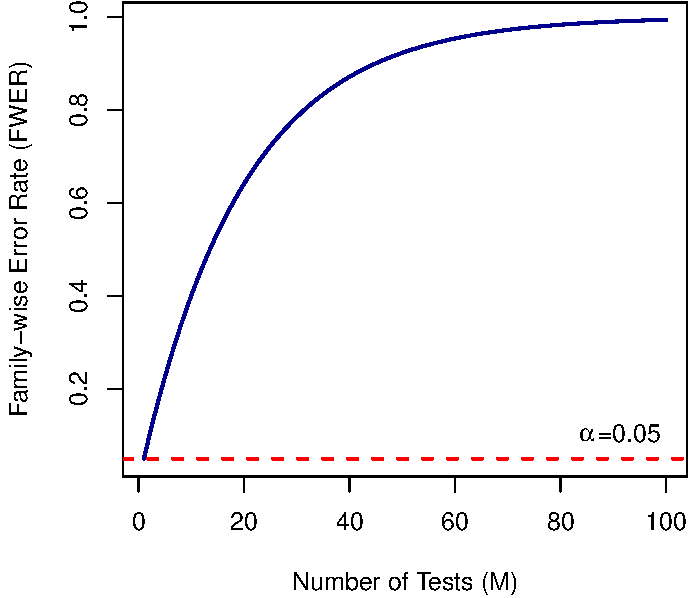
\includegraphics[width=0.5\textwidth]{FWER.pdf}
                  \caption{Family-Wise Error Rate Versus the Number of Hypothesis Tests, $M$.}\label{fig:FWER}
            \end{figure}
      \item A common value of $ M $ is $ \binom{m}{2} $: the number of pairwise comparisons necessary to compare each condition
            to every other condition.
            \begin{Example}{}{}
                  If $ m=5 $ and $ \alpha=0.05 $, then $ M=\binom{5}{2}=10 $. Therefore, $ \FWER=1-(1-0.05)^{10}=0.4013 $.
            \end{Example}
      \item Available to us are a variety of different statistical techniques that may be used to ensure the FWER
            does not exceed some threshold.
            \[ \FWER\le \alpha^\star \in[0,1] \]
            \begin{Remark}{General Notation}{}
                  \begin{itemize}
                        \item Denote the $ M $ null hypotheses as: $ \mathbf{H}_{0,1},\mathbf{H}_{0,2},\ldots,\mathbf{H}_{0,M} $.
                        \item Denote their corresponding $ p $-values as: $ p_1,p_2,\ldots,p_M $.
                  \end{itemize}
            \end{Remark}
            \begin{Example}{}{}
                  Suppose we test $ M =4 $ hypotheses, and the resulting $ p $-values are $ p_1 =0.015$, $ p_2=0.029 $,
                  $ p_3=0.008 $, and $ p_4=0.026 $.
            \end{Example}
\end{itemize}
\subsubsection*{The Bonferroni Correction}
\begin{itemize}
      \item This is the simplest method.
      \item Reject $ \mathbf{H}_{0,k} $ if
            \[ p_k\le \frac{\alpha^\star}{M} \quad\text{for }k=1,2,\ldots,M \]
            So, we test all $ M $ hypotheses at a significance level of $ \alpha^\star/M $.
      \item The procedure ensures $ \FWER\le \alpha^\star $. From Boole's Inequality,
            we know that
            \[ \FWER\le M\biggl(\frac{\alpha^\star}{M}\biggr)=\alpha^\star \]
      \item If we assume independence, the Bonferroni-corrected FWER becomes
            \[ 1-\biggl(1-\frac{\alpha^\star}{M} \biggr)^{\! M} \]
            Taking the limit of $ M \to\infty $ yields,
            \[ \lim\limits_{{M} \to {\infty}}\Biggl[1-\biggl(1-\frac{\alpha^\star}{M} \biggr)^{\! M}\Biggr]=1-e^{-\alpha^\star}  \]
            which for typical values of $ \alpha^\star $ in the range of $ \interval[open left]{0}{0.1} $ is approximately equal to $ \alpha^\star $.
            For example, if $ \alpha^\star=0.1 $, then the error is $ \approx 0.005 $. The asymptotic error rate
            and line of equality can be seen in~\Cref{fig:asymrate}.
            \begin{figure}[!htbp]
                  \centering
                  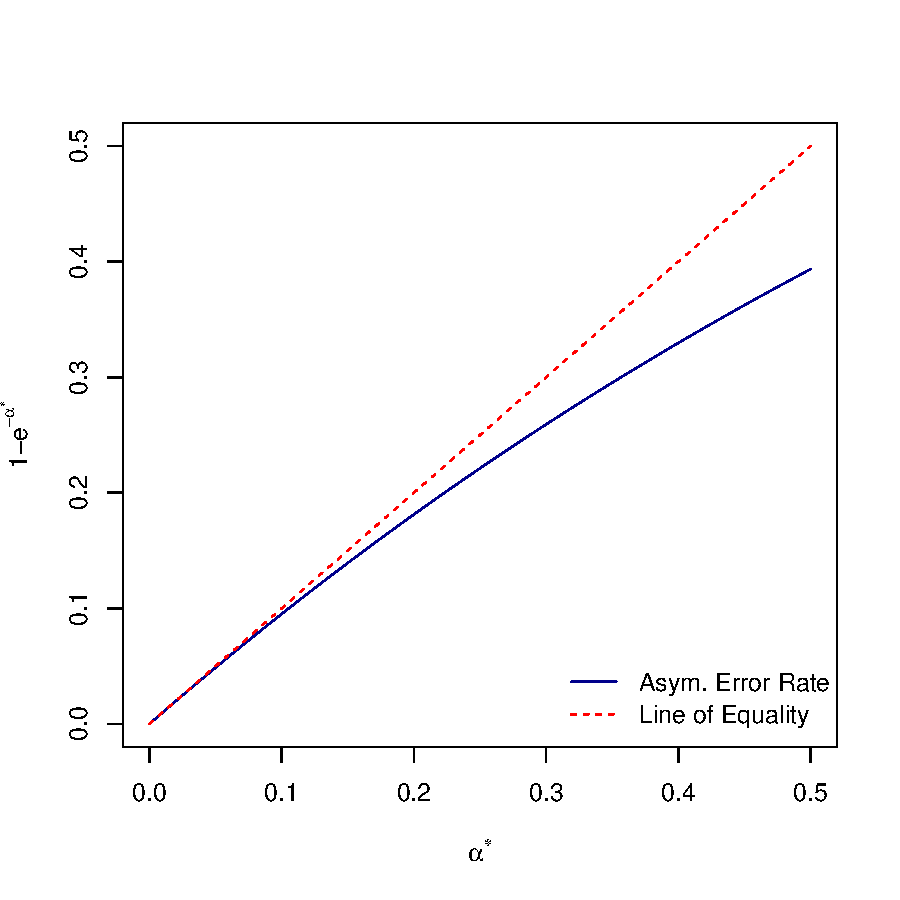
\includegraphics[width=0.5\textwidth]{asymrate.pdf}
                  \caption{Illustration of the Bonferroni Correction for Asymptotically Large $M$.}\label{fig:asymrate}
            \end{figure}
\end{itemize}
\begin{Example}{Four-test Example --- Bonferroni Correction}{}
      Let $ p_1=0.015 $, $ p_2=0.029 $, $ p_3=0.008 $, and $ p_4=0.026 $. Suppose that we wish to ensure
      $ \FWER\le \alpha^\star=0.05 $.

      \vspace{2mm}

      Under the Bonferroni Correction, we compare each
      $ p $-value to $ \alpha^\star/M=0.05/4=0.0125 $. Only $ p_3<0.0125 $, and hence
      only $ \mathbf{H}_{0,3} $ is rejected.
\end{Example}
\subsubsection*{The Šidák Correction}
\begin{itemize}
      \item This approach exploits the FWER formula derived when we assumed the $M$ tests were independent.
      \item Reject $ \mathbf{H}_{0,k} $ if
            \[ p_k\le 1-(1-\alpha^\star)^{1/M}\quad\text{for }k=1,2,\ldots,M \]
            \begin{Remark}{}{}
                  Where does the Šidák Correction come from?
                  \begin{align*}
                        \alpha^\star=\FWER=1-(1-\alpha)^M
                         & \iff 1-\alpha^\star = (1-\alpha)^M   \\
                         & \iff (1-\alpha^\star)^{1/M}=1-\alpha \\
                         & \iff \alpha=1-(1-\alpha^\star)^{1/M} \\
                  \end{align*}
            \end{Remark}
      \item This is actually not much different from the Bonferroni correction since
            \[ \frac{\alpha^\star}{M} \approx 1-(1-\alpha^\star)^{1/M} \]
            \begin{Example}{Bonferroni versus Šidák Correction}{}
                  Let $ \alpha^\star=0.05 $ and $ M=10 $. Then,
                  \[ \frac{\alpha^\star}{M} =0.005\quad\text{and}\quad 1-(1-\alpha^\star)^{1/M}=0.005116 \]
            \end{Example}
\end{itemize}
\begin{Example}{Four-test Example --- Šidák Correction}{}
      Let $ p_1=0.015 $, $ p_2=0.029 $, $ p_3=0.008 $, and $ p_4=0.026 $. Suppose that we wish to ensure
      $ \FWER\le \alpha^\star=0.05 $.

      \vspace{2mm}

      Under the Šidák Correction, we have
      \[ 1-(1-\alpha^\star)^{1/M}=1-(0.95)^{0.25}=0.012741 \]
      Therefore, we only reject $ \mathbf{H}_{0,3} $ since only $ p_3<0.012741 $.
\end{Example}
\subsubsection*{Holm's ``Step-Up'' Procedure}
\begin{itemize}
      \item The Bonferroni and Šidák corrections methods are very strict for large $M$.
            \begin{itemize}
                  \item In these cases \emph{most} null hypotheses will not be rejected.
                  \item If we're too strict, we basically stop rejecting null hypotheses thereby
                        eliminating Type I Errors, but we increase the Type II Errors.
            \end{itemize}
      \item Ideally we would have an approach that is less strict but still controls the FWER at some $ \alpha^\star $.
      \item This is exactly what Holm's Procedure gives us!
            \begin{framed}
                  \begin{enumerate}
                        \item Order the $M$ $p$-values from smallest to largest:
                              \[ p_{(1)},p_{(2)},\ldots,p_{(M)} \]
                              where $ p_{(k)} $ is the $ k^{\text{th}} $ smallest $ p $-value.
                        \item Starting from $ k=1 $ and continuing incrementally, compare
                              $ p_{(k)} $ to $ \alpha^\star/(M-k+1) $. Determine $ k^\star $,
                              the smallest value of $ k $ such that
                              \[ p_{(k)}>\frac{\alpha^\star}{M-k+1} \]
                        \item Reject the null hypotheses $ \mathbf{H}_{0,(1)},\ldots,\mathbf{H}_{0,(k^\star-1)} $
                              and do not reject $ \mathbf{H}_{0,(k^\star)},\ldots,\mathbf{H}_{0,(M)} $.
                  \end{enumerate}
            \end{framed}
      \item What's really happening?
            \begin{align*}
                  p_{(1)} & \text{ versus } \alpha^\star/M     \\
                  p_{(2)} & \text{ versus } \alpha^\star/(M-1) \\
                  p_{(3)} & \text{ versus } \alpha^\star/(M-2) \\
                          & \quad\;\vdots                      \\
                  p_{(M)} & \text{ versus } \alpha^\star
            \end{align*}
            We compare each $ p $-value to a Bonferroni-Corrected significance
            level based on the number of comparisons that remain to be
            made at a particular ``step.''
\end{itemize}
\begin{Theorem}{}{holm_FWER}
      Holm's procedure controls the family-wise error rate.
\end{Theorem}
\begin{Proof}{\Cref{thm:holm_FWER} \dagger}{}
      \begin{itemize}
            \item We need to show that $ \FWER=\Prob{V\ge 1}\le \alpha^\star\in[0,1] $ when using the Holm's procedure.
            \item Let $ p_{(1)},p_{(2)},\ldots,p_{(M)} $ be the ordered $ p $-values and let
                  $ \mathbf{H}_{0,(1)},\mathbf{H}_{0,(2)},\ldots,\mathbf{H}_{0,(M)} $ be the corresponding null hypotheses.
            \item Define $ K_0\subset \set{1,2,\ldots,M} $ to be the subset of indices which correspond
                  to true null hypotheses; that is, $ \mathbf{H}_{0,k} $ is true for $ k\in K_0 $.
            \item We can visualize the sequential decisions made in Holm's Procedure as follows:
                  \[ \overbracket{\underbracket{\mathbf{H}_{0,(1)}\cdots\mathbf{H}_{0,(h-1)}}_{\text{these are false $\mathbf{H}_0$'s}}\mathbf{H}_{0,(h)}\cdots \mathbf{H}_{0,(R)}}^{\text{these are rejected}}\mid \underbracket{\mathbf{H}_{0,(R+1)}\cdots\mathbf{H}_{0,(M)}}_{\text{these are not rejected}} \]
      \end{itemize}
      Let $ \mathbf{H}_{0,(h)} $ be the first \emph{true} $ \mathbf{H}_0 $ that was rejected. Since it was rejected by Holm's procedure, we know that
      \[ p_{(h)}\le \frac{\alpha^\star}{M-h+1} \]
      Also, clearly we must have $ h-1\le M-M_0 $ since $ M-M_0 $ is the total number of false $ \mathbf{H}_0 $'s and $ h-1 $ is the number of false
      $ \mathbf{H}_0 $'s encountered by test $ h $. And so,
      \[
            M_0\le M-h+1
            \iff \frac{1}{M_0} \ge \frac{1}{M-h+1}
            \iff \frac{\alpha^\star}{M_0} \ge \frac{\alpha^\star}{M-h+1}
      \]
      Thus, we must have $ p_{(h)}\le \alpha^\star/(M-h+1)\le \alpha^\star/M_0 $. Therefore,
      \begin{align*}
            \FWER
             & =\Prob*{V\ge 1}                                                                                                                    \\
             & =\Prob*{\text{At least one Type I Error in $M$ tests}}                                                                             \\
             & =\Prob*{\text{Reject at least one true $\mathbf{H}_0$}}                                                                            \\
             & =\Prob*{\exists\, k\in K_0\text{ such that }p_k\le \frac{\alpha^\star}{M_0}}                                                       \\
             & =\Prob*{\bigcup_{k\in K_0}p_k\le \frac{\alpha^\star}{M_0}}                                                                         \\
             & \le \sum_{k\in K_0}\Prob*{p_k\le \frac{\alpha^\star}{M_0}}                   &  & \text{by Boole's Inequality}                     \\
             & =\sum_{k\in K_0}\frac{\alpha^\star}{M_0}                                     &  & \!\!\!\!\begin{tabular}{l}
                  \text{since $p$-values for true null} \\
                  \text{hypotheses follow a $\uniform{0,1}$ distribution}
            \end{tabular}               \\
             & =M_0\biggl(\frac{\alpha^\star}{M_0}\biggr)                                   &  & \text{since the set $K_0$ has cardinality $M_0$} \\
             & =\alpha^\star
      \end{align*}
      Therefore, $ \FWER\le \alpha^\star $ as required.
\end{Proof}
\begin{Example}{Four-test Example ($ M=4 $) --- Holm's Procedure}{}
      Let $ p_1=0.015 $, $ p_2=0.029 $, $ p_3=0.008 $, and $ p_4=0.026 $. Suppose that we wish to ensure
      $ \FWER\le \alpha^\star=0.05 $.
      \begin{align*}
            p_{(1)}=p_3=0.008 & \text{ versus } \alpha^\star/M=0.05/4=0.0125     \\
            p_{(2)}=p_1=0.015 & \text{ versus } \alpha^\star/(M-1)=0.05/3=0.0167 \\
            p_{(3)}=p_4=0.026 & \text{ versus } \alpha^\star/(M-2)=0.05/2=0.025  \\
            p_{(4)}=p_2=0.029 & \text{ versus } \alpha^\star/(M-3)=0.05/1=0.05
      \end{align*}
      We reject $ \mathbf{H}_{0,(1)}=\mathbf{H}_{0,3} $ and $ \mathbf{H}_{0,(2)}=\mathbf{H}_{0,1} $. We do not reject
      $ \mathbf{H}_{0,(3)}=\mathbf{H}_{0,4} $ or $ \mathbf{H}_{0,(4)}=\mathbf{H}_{0,2} $. Note that $ k^\star=3 $.
\end{Example}
\begin{itemize}
      \item The decision process for all three of these methods can be visualized by plotting the ordered $p$-values
            $ p_{(k)} $ versus their ranks $ k=1,2,\ldots,M $ and overlay the significance thresholds which can
            be seen in~\Cref{fig:pvsrank1}.
            \begin{figure}[!htbp]
                  \centering
                  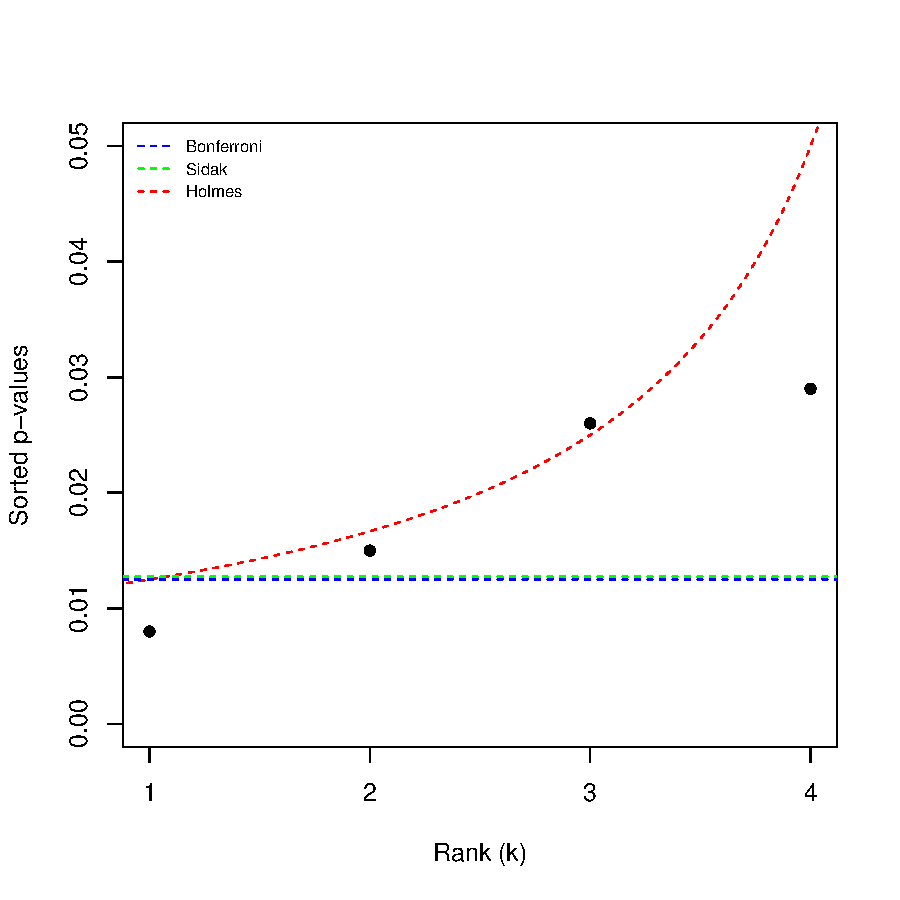
\includegraphics[width=0.5\textwidth]{pvsrank1.pdf}
                  \caption{Significance Thresholds for Several Methods of Correction (1).}\label{fig:pvsrank1}
            \end{figure}
      \item The Bonferroni correction is most strict, followed by the Šidák correction, then by Holm's procedure.
\end{itemize}
\subsubsection*{Adjusted $ p $-values}
\begin{itemize}
      \item So far we have framed each of the correction procedures above as an adjustment to the significance
            threshold against which each $p$-value is compared.
      \item Alternatively (and equivalently) we could invert this process and frame the decision in terms of a
            comparison of \emph{adjusted $p$-values} to $ \alpha^\star $.
      \item This is more familiar (compare our $ p $-values to some constant threshold $ \alpha^\star $).
            \begin{itemize}
                  \item We just need to adjust our $p$-values first.
            \end{itemize}
      \item The decisions made with the following adjusted $p$-values are identical to that achieved by comparing
            unadjusted $p$-values to the methods' adjusted significance thresholds.
            \begin{itemize}
                  \item Bonferroni: Reject $ \mathbf{H}_{0,k} $ if $ p_k^\star\le \alpha^\star $ where
                        \[ p_k^\star=Mp_k \]
                        \begin{Example}{Bonferroni's Adjusted $ p $-values}{}
                              In our four-test example, $ p_1^\star=0.06 $, $ p_2^\star=0.116 $, $ p_3^\star=0.032 $, and $ p_4^\star=0.104 $.
                              Comparing to $ \alpha^\star=0.05 $, we reject $ \mathbf{H}_{0,3} $.
                        \end{Example}
                  \item Šidák: Reject $ \mathbf{H}_{0,k} $ if $ p_k^\star\le \alpha^\star $ where
                        \[ p_k^\star=1-(1-p_k)^M \]
                        \begin{Example}{Šidák's Adjusted $ p $-values}{}
                              In our four-test example, $ p_1^\star=0.0587 $, $ p_2^\star=0.111 $, $ p_3^\star=0.0316 $, and $ p_4^\star=0.1 $.
                              Comparing to $ \alpha^\star=0.05 $, we reject $ \mathbf{H}_{0,3} $.
                        \end{Example}
                  \item Holm: Reject $ \mathbf{H}_{0,k} $ if $ p_{(k)}^\star\le \alpha^\star $ where
                        \[ p_{(k)}^\star=\max_{j\le k}\set*{p_{(j)}(M-j+1)} \]
                        \begin{Example}{Holm's Adjusted $ p $-values}{}
                              Let $ p_1=0.015 $, $ p_2=0.029 $, $ p_3=0.008 $, and $ p_4=0.026 $.
                              \[ \begin{array}{ccccl}
                                          k & p_{(k)} & M-k+1 & p_{(k)}(M-k+1) & p_{(k)}^\star=\max_{j\le k}\set*{p_{(j)}(M-j+1)}      \\
                                          \midrule
                                          1 & 0.008   & 4     & 0.032          & \max\set{0.032}=0.032=p_{(1)}^\star                   \\
                                          2 & 0.015   & 3     & 0.045          & \max\set{0.032,0.045}=0.045=p_{(2)}^\star             \\
                                          3 & 0.026   & 2     & 0.052          & \max\set{0.032,0.045,0.052}=0.052=p_{(3)}^\star       \\
                                          4 & 0.029   & 1     & 0.029          & \max\set{0.032,0.045,0.052,0.029}=0.052=p_{(4)}^\star
                                    \end{array} \]
                              Thus, $ p_1^\star=p_{(2)}^\star=0.045 $, $ p_2^\star=p_{(4)}^\star=0.052 $, $ p_3^\star=p_{(1)}^\star=0.032 $, and
                              $ p_4^\star=p_{(3)}^\star=0.052 $. Comparing to $ \alpha^\star=0.05 $, we reject
                              $ \mathbf{H}_{0,1} $ and $ \mathbf{H}_{0,3} $.
                        \end{Example}
            \end{itemize}
      \item Implemented in R with \code{p.adjust()}.
\end{itemize}
\subsection{False Discovery Rate}
\begin{itemize}
      \item In the mid-1900s, Statisticians developed FWER methods with $ M\approx 20 $ comparisons in mind.
      \item In the era of Big Data, much larger values of $M$ are typical.
      \item For larger values of $M$, traditional methods tend to be very conservative, and so FWER is perhaps
            not the best metric to control.
      \item More recently, emphasis has been placed on controlling the \emph{rate} at which Type I Errors occur.
            \begin{Definition}{False discovery proportion}{}
                  The \textbf{false discovery proportion} (FDP) is
                  \[ Q=\frac{V}{R} \]
                  Thus, $ Q $ is the proportion of all rejected null hypotheses that were rejected
                  in error.
            \end{Definition}
      \item In particular, interest lies in controlling the \textbf{false discovery rate} (FDR).
            \begin{Definition}{False discovery rate}{}
                  The \textbf{false discovery rate} is
                  \[ \E{Q}=\E*{\frac{V}{R}} \]
            \end{Definition}
      \item Unlike the FWER, the FDR is adaptive in the sense that the number of Type I Errors $V$ has different
            implications depending on the size of $M$. That is,
            \begin{itemize}
                  \item Two Type I Errors in 10 tests might be unacceptable.
                  \item Two Type I Errors in 100 tests might be okay.
            \end{itemize}
      \item Methods that control the FDR are less strict than methods that control FWER\@.
            \begin{itemize}
                  \item More Type I Errors will occur with such methods, but this is viewed as acceptable when $M$ is
                        very large.
            \end{itemize}
\end{itemize}
\subsubsection*{Benjamini-Hochberg Procedure}
\begin{itemize}
      \item The Benjamini-Hochberg (BH) procedure for controlling FDR is a sequentially rejective procedure
            much like Holm's procedure for controlling FWER\@. The main difference is the threshold we
            compare the ordered $ p $-values to.
      \item We summarize the BH procedure, which aims to ensure $ \text{FDR}\le \alpha^\star $:
            \begin{framed}
                  \begin{enumerate}
                        \item Order the $M$ $p$-values from smallest to largest:
                              \[ p_{(1)},p_{(2)},\ldots,p_{(M)} \]
                              where $ p_{(k)} $ is the $ k^{\text{th}} $ smallest $ p $-value.
                        \item Starting from $ k=1 $ and continuing incrementally, compare
                              $ p_{(k)} $ to $ k\alpha^\star/M $. Determine $ k^\star $
                              the largest value of $ k $ such that
                              \[ p_{(k)}\le \frac{k\alpha^\star}{M}  \]
                        \item Reject the null hypotheses $ \mathbf{H}_{0,(1)},\ldots,\mathbf{H}_{0,(k^\star)} $
                              and do not reject $ \mathbf{H}_{0,(k^\star+1)},\ldots,\mathbf{H}_{0,(M)} $.
                  \end{enumerate}
            \end{framed}
      \item The decision process associated with this procedure is best visualized with a plot of the ordered $p$-values
            $ p_{(k)} $ versus their ranks $ k=1,2,\ldots,M $ with the significance threshold overlaid which can
            be seen in~\Cref{fig:pvsrank2}.
            \begin{itemize}
                  \item The BH significance threshold is the line with intercept $0$ and slope $ \alpha^\star/M $.
            \end{itemize}
            \begin{figure}[!htbp]
                  \centering
                  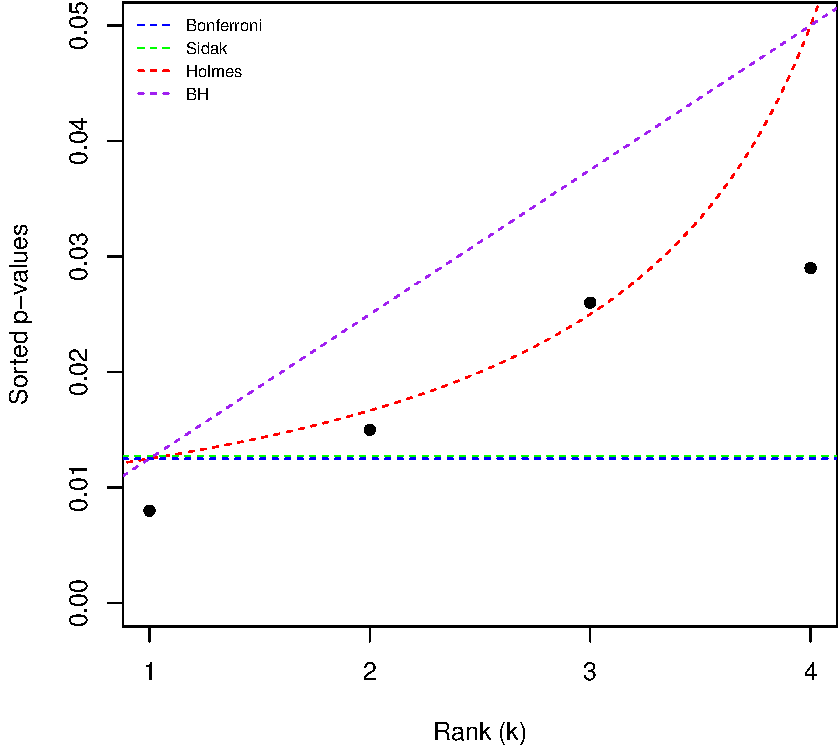
\includegraphics[width=0.5\textwidth]{pvsrank2.pdf}
                  \caption{Significance Thresholds for Several Methods of Correction (2).}\label{fig:pvsrank2}
            \end{figure}
            \begin{Example}{Four-test Example --- Benjamini-Hochberg Procedure}{}
                  Let $ p_1=0.015 $, $ p_2=0.029 $, $ p_3=0.008 $, and $ p_4=0.026 $. Suppose that we wish to ensure
                  $ \FWER\le \alpha^\star=0.05 $. Since all $ p $-values fall below the purple line in~\Cref{fig:pvsrank2},
                  we reject all four null hypotheses.
            \end{Example}
      \item This threshold is much less strict than any of the FWER-control thresholds, but this is the appeal of
            the approach.
      \item The procedure that guarantees $ \text{FDR}\le \alpha^\star $ is beyond the scope of this course.
            However, the proof can be found in~\citet{benjamini} and~\citet{storey}.
      \item Like the FWER controlling methods we can define Benjamini-Hochberg-adjusted $p$-values and invert
            the decision framework by comparing the adjusted $ p $-values to $ \alpha^\star $.
            \begin{itemize}
                  \item Reject $ \mathbf{H}_{0,(k)} $ if $ p_{(k)}^\star\le \alpha^\star $ where
                        \[ p_{(k)}^\star=\min_{j\ge k}\set*{\frac{Mp_{(j)}}{j}} \]
                        \begin{Example}{Benjamini-Hochberg Procedure's Adjusted $ p $-values}{}
                              Let $ p_1=0.015 $, $ p_2=0.029 $, $ p_3=0.008 $, and $ p_4=0.026 $.
                              \[ \begin{array}{cccl}
                                          k & p_{(k)} & M p_{(k)}/k & p_{(k)}^\star=\min_{j\ge k}\set*{Mp_{(j)}/j}          \\
                                          \midrule
                                          1 & 0.008   & 0.032       & \min\set{0.032,0.030,0.035,0.029}=0.029=p_{(1)}^\star \\
                                          2 & 0.015   & 0.030       & \min\set{0.030,0.035,0.029}=0.029=p_{(2)}^\star       \\
                                          3 & 0.026   & 0.035       & \min\set{0.035,0.029}=0.029=p_{(3)}^\star             \\
                                          4 & 0.029   & 0.029       & \min\set{0.029}=0.029=p_{(4)}^\star
                                    \end{array} \]
                              Thus, $ p_1^\star=p_{(2)}^\star=0.029 $, $ p_2^\star=p_{(4)}^\star=0.029 $, $ p_3^\star=p_{(1)}^\star=0.029 $,
                              and $ p_4^\star=p_{(3)}^\star=0.029 $. Comparing to $ \alpha^\star=0.05 $,
                              we reject all $ \mathbf{H}_{0} $'s.
                        \end{Example}
            \end{itemize}
\end{itemize}
\href{https://github.com/Hextical/university-notes/blob/master/year-3/semester-3/STAT 430/code/Multiple_testing_example.R}{[R Code] \texttt{Multiple\_testing\_example}}
\subsection{Sample Size Determination}
\begin{itemize}
      \item So what does all of this mean for power analyses and sample size calculations?
      \item There is a duality between significance level and power.
            \begin{itemize}
                  \item All else equal, reducing a test's significance level will increase the Type II Error rate and hence
                        decrease power.
                  \item Play around with \href{https://nathaniel-t-stevens.shinyapps.io/ErrorIllustrator/}{this interactive app} to gain comfort with this notion.
                        \begin{itemize}
                              \item Assume $ \mathcal{R}=\set*{t\mid t\ge z_\alpha} $.
                              \item Recall that: \begin{itemize}
                                          \item $ \alpha=\Prob*{\text{Type I Error}}=\Prob*{T\in\mathcal{R}\given \text{$ \mathbf{H}_0 $ is true}}=\Prob*{T\ge z_\alpha\given \text{$ \mathbf{H}_0 $ is true}}$.
                                          \item $ \beta=\Prob*{\text{Type II Error}}=\Prob*{T\notin\mathcal{R}\given \text{$ \mathbf{H}_\text{A} $ is true}}=\Prob*{T< z_\alpha\given \text{$ \mathbf{H}_\text{A} $ is true}} $.
                                    \end{itemize}
                        \end{itemize}
            \end{itemize}
      \item Thus, all the correction procedures discussed (which decrease the effective significance level)
            negatively impact power.
      \item In order to maintain power at some pre-specified level, we must compensate by increasing the sample
            size.
      \item Therefore, the more complicated your experiment (i.e., the more conditions it has), the larger your
            sample sizes will need to be.
            \begin{itemize}
                  \item Such modifications can be accounted for when selecting a sample size.
                  \item The significance level you use in your sample size calculations should be the adjusted one based
                        on the correction method you use.
                  \item This is easier to do with \emph{some} correction methods than others.
            \end{itemize}
\end{itemize}
